\documentclass{suftesi}
\usepackage{geometry}
\usepackage{graphicx}
\usepackage[backend=biber, style=alphabetic]{biblatex}
\let\openbox\relax
\usepackage{amsmath, amsthm}
\usepackage{enumitem}
\usepackage{float}
\usepackage[ruled]{algorithm2e}
\usepackage{titlesec}
\usepackage{mathtools}
\usepackage{stmaryrd}
\titleformat{\section}[hang]{\normalfont\fontsize{11}{16}\bfseries}{\thesection}{1em}{}
\addbibresource{/Users/giuseppe/Desktop/Master of Logic/First year/Third Period/Project_STL/references.bib}
\newtheorem*{definition}{Definition}
\newtheorem*{proposition}{Proposition}

 \usepackage{tikz}
 \DeclareSymbolFont{symbolsC}{U}{txsyc}{m}{n}
\SetSymbolFont{symbolsC}{bold}{U}{txsyc}{bx}{n}

\DeclareMathSymbol{\rightfishhook}{\mathrel}{symbolsC}{"4A}
\DeclareMathSymbol{\leftfishhook}{\mathrel}{symbolsC}{"4B}
\DeclareMathSymbol{\leftrightfishhook}{\mathrel}{symbolsC}{"4C}

\DeclareMathSymbol{\boxrightarrow}{\mathrel}{symbolsC}{"80}
\DeclareMathSymbol{\boxleftarrow}{\mathrel}{symbolsC}{"81}
\DeclareMathSymbol{\boxdotrightarrow}{\mathrel}{symbolsC}{"82}
\DeclareMathSymbol{\boxdotleftarrow}{\mathrel}{symbolsC}{"83}
\newcommand{\boxleftrightarrow}{\mathrlap{\boxleftarrow}\mspace{8.75mu}\boxrightarrow}
\newcommand{\boxdotleftrightarrow}{\mathrlap{\boxdotleftarrow}\mspace{8.75mu}\boxdotrightarrow}

\DeclareMathSymbol{\diamondrightarrow}{\mathrel}{symbolsC}{"84}
\DeclareMathSymbol{\diamondleftarrow}{\mathrel}{symbolsC}{"85}
\DeclareMathSymbol{\diamonddotrightarrow}{\mathrel}{symbolsC}{"86}
\DeclareMathSymbol{\diamonddotleftarrow}{\mathrel}{symbolsC}{"87}
\newcommand{\diamondleftrightarrow}{\mathrlap{\diamondleftarrow}\mspace{6.5mu}\diamondrightarrow}
\newcommand{\diamonddotleftrightarrow}{\mathrlap{\diamonddotleftarrow}\mspace{6.5mu}\diamonddotrightarrow}

\DeclareMathSymbol{\boxRightarrow}{\mathrel}{symbolsC}{"88}
\DeclareMathSymbol{\boxLeftarrow}{\mathrel}{symbolsC}{"89}
\DeclareMathSymbol{\boxdotRightarrow}{\mathrel}{symbolsC}{"8A}
\DeclareMathSymbol{\boxdotLeftarrow}{\mathrel}{symbolsC}{"8B}
\newcommand{\boxLeftrightarrow}{\mathrlap{\boxLeftarrow}\mspace{8.75mu}\boxRightarrow}
\newcommand{\boxdotLeftrightarrow}{\mathrlap{\boxdotLeftarrow}\mspace{8.75mu}\boxdotRightarrow}

\DeclareMathSymbol{\diamondRightarrow}{\mathrel}{symbolsC}{"8C}
\DeclareMathSymbol{\diamondLeftarrow}{\mathrel}{symbolsC}{"8D}
\DeclareMathSymbol{\diamonddotRightarrow}{\mathrel}{symbolsC}{"8E}
\DeclareMathSymbol{\diamonddotLeftarrow}{\mathrel}{symbolsC}{"8F}
\newcommand{\diamondLeftrightarrow}{\mathrlap{\diamondLeftarrow}\mspace{6.5mu}\diamondRightarrow}
\newcommand{\diamonddotLeftrightarrow}{\mathrlap{\diamonddotLeftarrow}\mspace{6.5mu}\diamonddotRightarrow}

\DeclareMathSymbol{\circlerightarrow}{\mathrel}{symbolsC}{"91}
\DeclareMathSymbol{\circleleftarrow}{\mathrel}{symbolsC}{"92}
\DeclareMathSymbol{\circledotrightarrow}{\mathrel}{symbolsC}{"93}
\DeclareMathSymbol{\circledotleftarrow}{\mathrel}{symbolsC}{"94}
\newcommand{\circleleftrightarrow}{\mathrlap{\circleleftarrow}\mspace{7.25mu}\circlerightarrow}
\newcommand{\circledotleftrightarrow}{\mathrlap{\circledotleftarrow}\mspace{7.25mu}\circledotrightarrow}

% MnSymbol C
\DeclareFontFamily{U}  {MnSymbolC}{}
\DeclareFontShape{U}{MnSymbolC}{m}{n}{
    <-6>  MnSymbolC5
   <6-7>  MnSymbolC6
   <7-8>  MnSymbolC7
   <8-9>  MnSymbolC8
   <9-10> MnSymbolC9
  <10-12> MnSymbolC10
  <12->   MnSymbolC12}{}

\DeclareFontShape{U}{MnSymbolC}{b}{n}{
    <-6>  MnSymbolC-Bold5
   <6-7>  MnSymbolC-Bold6
   <7-8>  MnSymbolC-Bold7
   <8-9>  MnSymbolC-Bold8
   <9-10> MnSymbolC-Bold9
  <10-12> MnSymbolC-Bold10
  <12->   MnSymbolC-Bold12}{}

\DeclareSymbolFont{MnSyC}         {U}  {MnSymbolC}{m}{n}
\SetSymbolFont{MnSyC}       {bold}{U}  {MnSymbolC}{b}{n}

\DeclareMathSymbol{\medtriangleright}{\mathrel}{MnSyC}{80}
\DeclareMathSymbol{\medtriangleup}{\mathrel}{MnSyC}{81}
\DeclareMathSymbol{\medtriangleleft}{\mathrel}{MnSyC}{82}
\DeclareMathSymbol{\medtriangledown}{\mathrel}{MnSyC}{83}
\DeclareMathSymbol{\medtrianglerightfilled}{\mathrel}{MnSyC}{200}
\DeclareMathSymbol{\medtriangleupfilled}{\mathrel}{MnSyC}{201}
\DeclareMathSymbol{\medtriangleleftfilled}{\mathrel}{MnSyC}{202}
\DeclareMathSymbol{\medtriangledownfilled}{\mathrel}{MnSyC}{203}


\DeclareMathSymbol{\medcircle}{\mathrel}{MnSyC}{90}
\DeclareMathSymbol{\medcircleminus}{\mathrel}{MnSyC}{92}
\DeclareMathSymbol{\medcirclevert}{\mathrel}{MnSyC}{93}
\DeclareMathSymbol{\medcircleplus}{\mathrel}{MnSyC}{96}
\DeclareMathSymbol{\medcircletimes}{\mathrel}{MnSyC}{97}
\DeclareMathSymbol{\medcircledot}{\mathrel}{MnSyC}{98}
\DeclareMathSymbol{\bullet}{\mathrel}{MnSyC}{89}
\newcommand{\medcirclefilled}{\text{\raisebox{-0.2ex}{\scalebox{1.5}{\ensuremath{\bullet}\xspace}}}}

\DeclareMathSymbol{\medsquare}{\mathrel}{MnSyC}{106}
\DeclareMathSymbol{\medsquareminus}{\mathrel}{MnSyC}{112}
\DeclareMathSymbol{\medsquarevert}{\mathrel}{MnSyC}{113}
\DeclareMathSymbol{\medsquareplus}{\mathrel}{MnSyC}{116}
\DeclareMathSymbol{\medsquaretimes}{\mathrel}{MnSyC}{117}
\DeclareMathSymbol{\medsquaredot}{\mathrel}{MnSyC}{118}
\DeclareMathSymbol{\medsquarefilled}{\mathrel}{MnSyC}{204}

\DeclareMathSymbol{\meddiamond}{\mathrel}{MnSyC}{110}
\DeclareMathSymbol{\meddiamondminus}{\mathrel}{MnSyC}{120}
\DeclareMathSymbol{\meddiamondvert}{\mathrel}{MnSyC}{121}
\DeclareMathSymbol{\meddiamondplus}{\mathrel}{MnSyC}{124}
\DeclareMathSymbol{\meddiamondtimes}{\mathrel}{MnSyC}{125}
\DeclareMathSymbol{\meddiamonddot}{\mathrel}{MnSyC}{126}
\DeclareMathSymbol{\diamondfilled}{\mathrel}{MnSyC}{109}
\newcommand{\meddiamondfilled}{\text{\raisebox{-0.2ex}{\scalebox{1.5}{\ensuremath{\diamondfilled}\xspace}}}}

\DeclareMathSymbol{\medstar}{\mathrel}{MnSyC}{130}
\DeclareMathSymbol{\medpentagram}{\mathrel}{MnSyC}{132}
\DeclareMathSymbol{\filledlargestar}{\mathord}{MnSyC}{205}
\newcommand{\medstarfilled}{\text{\scalebox{0.7}{\ensuremath{\filledlargestar}}}}
\DeclareMathSymbol{\medstarofdavid}{\mathord}{MnSyC}{207}

% mathabx b
\DeclareFontFamily{U}{mathb}{\hyphenchar\font45}
\DeclareFontShape{U}{mathb}{m}{n}{
      <5> <6> <7> <8> <9> <10> gen * mathb
      <10.95> mathb10 <12> <14.4> <17.28> <20.74> <24.88> mathb12
      }{}
\DeclareSymbolFont{mathb}{U}{mathb}{m}{n}

\DeclareMathSymbol{\bigvarstar}{2}{mathb}{'17}

% Modal Operator Commands
%##############################
\newcommand{\modalop}[1]{\mathop{#1}\nolimits} % \nolimits so that subscripts and superscripts aren't placed over the symbol
\newcommand{\modalbin}[1]{\mathbin{#1}}

% Box Operators
%##############################
\newcommand{\boxmodal}[1]{\modalop{\text{\raisebox{-0.1ex}{\scalebox{1.3}{\ensuremath{#1}}}}}} % ensures correct sizing
\newcommand{\nec}{\boxmodal{\medsquare}}
\newcommand{\necd}{\boxmodal{\medsquaredot}}
\newcommand{\necf}{\boxmodal{\medsquarefilled}}
\newcommand{\necm}{\boxmodal{\medsquareminus}}
\newcommand{\necv}{\boxmodal{\medsquarevert}}
\newcommand{\necp}{\boxmodal{\medsquareplus}}
\newcommand{\necx}{\boxmodal{\medsquaretimes}}

% Diamond Operators
%##############################
\newcommand{\diamodal}[1]{\modalop{\text{\scalebox{1.1}{\ensuremath{#1}}}}}
\newcommand{\pos}{\diamodal{\meddiamond}}
\newcommand{\posd}{\diamodal{\meddiamonddot}}
\newcommand{\posf}{\diamodal{\meddiamondfilled}}
\newcommand{\posm}{\diamodal{\meddiamondminus}}
\newcommand{\posv}{\diamodal{\meddiamondvert}}
\newcommand{\posp}{\diamodal{\meddiamondplus}}
\newcommand{\posx}{\diamodal{\meddiamondtimes}}

% Counterfactuals
%##############################
\newcommand{\necif}{\modalbin{\boxrightarrow}}
\newcommand{\necfi}{\modalbin{\boxleftarrow}}
\newcommand{\neciff}{\modalbin{\boxleftrightarrow}}
\newcommand{\necIf}{\modalbin{\boxRightarrow}}
\newcommand{\necFi}{\modalbin{\boxLeftarrow}}
\newcommand{\necIff}{\modalbin{\boxLeftrightarrow}}

\newcommand{\necdif}{\modalbin{\boxdotrightarrow}}
\newcommand{\necdfi}{\modalbin{\boxdotleftarrow}}
\newcommand{\necdiff}{\modalbin{\boxdotleftrightarrow}}
\newcommand{\necdIf}{\modalbin{\boxdotRightarrow}}
\newcommand{\necdFi}{\modalbin{\boxdotLeftarrow}}
\newcommand{\necdIff}{\modalbin{\boxdotLeftrightarrow}}

\newcommand{\posif}{\modalbin{\diamondrightarrow}}
\newcommand{\posfi}{\modalbin{\diamondleftarrow}}
\newcommand{\posiff}{\modalbin{\diamondleftrightarrow}}
\newcommand{\posIf}{\modalbin{\diamondRightarrow}}
\newcommand{\posFi}{\modalbin{\diamondLeftarrow}}
\newcommand{\posIff}{\modalbin{\diamondLeftrightarrow}}

\newcommand{\posdif}{\modalbin{\diamonddotrightarrow}}
\newcommand{\posdfi}{\modalbin{\diamonddotleftarrow}}
\newcommand{\posdiff}{\modalbin{\diamonddotleftrightarrow}}
\newcommand{\posdIf}{\modalbin{\diamonddotRightarrow}}
\newcommand{\posdFi}{\modalbin{\diamonddotLeftarrow}}
\newcommand{\posdIff}{\modalbin{\diamonddotLeftrightarrow}}

\newcommand{\deoif}{\modalbin{\circlerightarrow}}
\newcommand{\deofi}{\modalbin{\circleleftarrow}}
\newcommand{\deoiff}{\modalbin{\circleleftrightarrow}}

\newcommand{\deodif}{\modalbin{\circledotrightarrow}}
\newcommand{\deodfi}{\modalbin{\circledotleftarrow}}
\newcommand{\deodiff}{\modalbin{\circledotleftrightarrow}}

% Strict Conditionals
%##############################
\let\strictif\relax
\let\strictfi\relax
\let\strictiff\relax
\newcommand{\strictif}{\modalbin{\rightfishhook}}
\newcommand{\strictfi}{\modalbin{\leftfishhook}}
\newcommand{\strictiff}{\modalbin{\leftrightfishhook}}

% Deontic Operators
%##############################
\newcommand{\deon}[1]{\modalop{#1}}
\newcommand{\ought}{\deon{O}}
\newcommand{\may}{\deon{M}}
\newcommand{\permit}{\deon{P}}

\newcommand{\circmodal}[1]{\modalop{\text{\raisebox{-0.05ex}{\scalebox{1.2}{\ensuremath{#1}}}}}}
\newcommand{\deo}{\circmodal{\medcircle}}
\newcommand{\deod}{\circmodal{\medcircledot}}
\newcommand{\deof}{\circmodal{\medcirclefilled}}
\newcommand{\deom}{\circmodal{\medcircleminus}}
\newcommand{\deov}{\circmodal{\medcirclevert}}
\newcommand{\deop}{\circmodal{\medcircleplus}}
\newcommand{\deox}{\circmodal{\medcircletimes}}

% Star Operators
%##############################
\let\smallstar\star
\let\star\relax
\newcommand{\star}{\modalop{\medstar}}
\newcommand{\starf}{\modalop{\text{\raisebox{0.15ex}{\medstarfilled}}}}
\newcommand{\stard}{\modalop{\text{\raisebox{0.15ex}{\scalebox{0.7}{\ensuremath{\medstarofdavid}}}}}}
\let\medstarvar\bigvarstar % from mathabx
\newcommand{\starv}{\modalop{\ensuremath{\medstarvar}}}
\newcommand{\starp}{\modalop{\medpentagram}}

% Triangle Operators
%##############################
\newcommand{\triupmodal}[1]{\modalop{\text{\raisebox{-0.2ex}{\scalebox{1.2}{\ensuremath{#1}}}}}}
\newcommand{\tri}{\triupmodal{\medtriangleup}}
\newcommand{\trif}{\triupmodal{\medtriangleupfilled}}

\newcommand{\tridownmodal}[1]{\modalop{\text{\raisebox{0.15ex}{\scalebox{1.2}{\ensuremath{#1}}}}}}
\newcommand{\trid}{\tridownmodal{\medtriangledown}}
\newcommand{\tridf}{\tridownmodal{\medtriangledownfilled}}

\newcommand{\trileftmodal}[1]{\modalop{\text{\raisebox{-0.05ex}{\scalebox{1.2}{\ensuremath{#1}}}}}}
\newcommand{\tril}{\trileftmodal{\medtriangleleft}}
\newcommand{\trilf}{\trileftmodal{\medtriangleleftfilled}}

\newcommand{\trirightmodal}[1]{\modalop{\text{\raisebox{-0.05ex}{\scalebox{1.2}{\ensuremath{#1}}}}}}
\newcommand{\trir}{\trirightmodal{\medtriangleright}}
\newcommand{\trirf}{\trirightmodal{\medtrianglerightfilled}}

\newenvironment{theorem}[2][Theorem]{\begin{trivlist}
\item[\hskip \labelsep {\bfseries #1}\hskip \labelsep {\bfseries #2.}]}{\end{trivlist}}
\newenvironment{lemma}[2][Lemma]{\begin{trivlist}
\item[\hskip \labelsep {\bfseries #1}\hskip \labelsep {\bfseries #2.}]}{\end{trivlist}}
\newenvironment{exercise}[2][Exercise]{\begin{trivlist}
\item[\hskip \labelsep {\bfseries #1}\hskip \labelsep {\bfseries #2.}]}{\end{trivlist}}
\newenvironment{problem}[2][Problem]{\begin{trivlist}
\item[\hskip \labelsep {\bfseries #1}\hskip \labelsep {\bfseries #2.}]}{\end{trivlist}}
\newenvironment{question}[2][Question]{\begin{trivlist}
\item[\hskip \labelsep {\bfseries #1}\hskip \labelsep {\bfseries #2.}]}{\end{trivlist}}
\newenvironment{corollary}[2][Corollary]{\begin{trivlist}
\item[\hskip \labelsep {\bfseries #1}\hskip \labelsep {\bfseries #2.}]}{\end{trivlist}}

\newenvironment{solution}{\begin{proof}[Solution]}{\end{proof}}

\renewcommand{\b}{\textbf}
\renewcommand{\i}{\textit}
\setlength\parindent{0pt}
\newcommand{\STL}{$\mathtt{STL}$ }
\newcommand{\TL}{$\mathtt{TL}$ }
\newcommand{\TFL}{$\mathtt{TFL}$ }
\newcommand{\MITL}{$\mathtt{MITL}$ }
\newcommand{\abs}[1]{\lvert #1 \rvert}
\newcommand{\sem}[1]{\llbracket #1 \rrbracket}
\newcommand{\dom}[1]{\mathrm{dom}(#1 ,w)}

\title{\textcolor{black}{Summary of the papers for the report}}
\author{}
\date{}

\begin{document}

\maketitle

\tableofcontents
\newpage
\setcounter{page}{1}

\chapter{\citetitle{donze2012}}

\b{Object}: Presentation of a new temporal logic for REAL-VALUED SIGNALS with a checking framework 

\STL = temporal logic proprieties + frequency-domain properties

Temporal Logic puts the focus on the ongoing input-output behavior of reactive systems, rather than the final output.

\begin{itemize}[leftmargin=3cm]
    \item [\b{Reactive systems} =] viewed by designers as networks of transducers (block diagrams) communicating continuously via signals.
\end{itemize}
\begin{itemize} [leftmargin=1.35cm]
    \item [\b{Signal} =] function from Time ($\mathbb{T}$) to Real numbers ($\mathbb{R}$)
\end{itemize}

\TL provides a framework to write in a formal way specifications that the system under design should satisfy. It has been used to specify proprieties of real-valued signals defined over dense time domains.

\STL allows designers to speak of proprieties relates to the order of discrete events and the temporal distance between them. 

\begin{itemize} [leftmargin=1.3cm]
    \item [\b{Event} =] change in the satisfaction of some predicate over the real variables.
\end{itemize}

Traditional measures for signals are more continuous and event-free: averages/discounted integrals of some variables over time.

One of the impediment to \STL was its purely time-domain nature that does not match with the frequency-domain analysis. Frequency-domain analysis is based on Fourier spectrum of the signal, that leave aside the time at which events occur. This is done to deal with \b{noise}.

\begin{itemize} [leftmargin=1.3cm]
    \item [\b{Noise} =] random perturbations in the designed signal, in the frequency domain dealt with filtering techniques.
    It populates range of frequencies different from the designed signal, and therefore we keep only the latter, then we reduce the noise (\i{separation of the source}).
\end{itemize}

These kinds of operations are time-invariant, since the Fourier transform is defined over an unbounded time-interval, i.e. $t\in(-\infty,+\infty)$.
If we have bounded intervals the Fourier transform is not so useful, since its definition aggregates for each frequency all values along the duration of the signal.

Therefore, the aim is to search for proper \b{time-frequency analysis techniques}. In this paper the authors try to do so by proposing a unified \b{logical formalism} for expressing hybrid proprieties of signals.

\section{SIGNAL TEMPORAL LOGIC}

Consider a general framework of data-flow systems and add the temporal operators (until and since) as a special type of signal transducers.

Style of presentation of the semantics using temporal testers, applied to translate \STL monitoring.

A formula $\varphi$ is a network of signal operator (transducers), starting with a raw signal $x$ (sequences of atomic propositions in the discrete case), and cumulating in a top-level signal $\varphi$, whose vale at $t$ represents the satisfaction of the top-level formula at time $t$:
$$\varphi[t]=1 \Leftrightarrow (x,t)\vDash \varphi$$

Each sub-formula of the form $\varphi=f(\psi_1, \psi_2)$ is associated with a signal transducer $f$ that takes as input the satisfaction signals of $\psi_1$ and $\psi_2$.

The apparatus of monitoring the satisfaction of a formula by a signal can be viewed as a network of operators working on 
\begin{itemize}[leftmargin=0.5cm]
    \item \b{numerical signals}: raw signals and those obtained by numerical operations on them,
    \item \b{Boolean signals}: satisfaction signals of sub-formulae.
\end{itemize}

Assume that the signals are defined as functions from time $\mathbb{T}$ to some domain $\mathcal{D}$, the range $\mathbb{T}$ can be finite $[0, r]$, infinite $[0, +\infty)$ or bi-infinite $(-\infty, +\infty)$.

\begin{definition}
    A signal operator is a mapping $f: (\mathbb{T}\to\mathcal{D}_1)\to(\mathbb{T}\to\mathcal{D}_2)$, where $\mathcal{D}_1$ and $\mathcal{D}_2$ are respectively domains of input and output signals.
\end{definition}

All the operators are computable so that given some representation of a signal $x$, we can produce a representation of the output signal $f(x)$.

\begin{definition}
    Let $f$ be a signal operator and let $y=f(x)$. We say that $f$ is:
    \begin{itemize}[leftmargin=0.5cm]
        \item \b{memoryless} if it is lifting to signals of a function $f: \mathcal{D}_1\to\mathcal{D}_2$, that is, $\forall t\,y[t]=f(x[t])$
        \item \b{casual} if for every $t$, $y[t]$ is computed based only on at most $x[0],\dots, x[t]$,
        \item \b{acasual} otherwise.
    \end{itemize}
\end{definition}

Casual operators: past operator, back-shifts or integral over temporal window that extend them. They can be monitored online, and it is important for real systems.

Acasual operators: future operator and operators and the ones depending on values in the temporal windows that extend beyond the current time. 

\begin{definition}
    Let $\varphi_1$ and $\varphi_2$ be two Boolean signals, and let $a,b\in\mathbb{R}$ such that $a\leq b$. Then $\psi=\varphi_1\,\mathcal{U}_{[a,b]}\,\varphi_2$ are signals satisfying: $$(x,t)\vDash\psi \Leftrightarrow\exists t'\in [a+t,b+t], (x,t')\vDash\varphi_2\:\land \:\forall t''\in[t,t'](x,t'')\vDash\varphi_1[t'']$$ 
\end{definition}

Since the Boolean operators `$\lor$' and `$\land$' are definable with $\min$ and $\max$. We can rewrite $\psi[t]$ as follows:
$$\psi[t]=\max_{t'\in[a+t,b+t]}\min(\min_{t''\in[t,t']}\varphi_1[t''],\varphi_2[t'])$$
    
We have the derived temporal operators $\pos_{[a,b]}\varphi = \top\,\mathcal{U}_{a,b}\,\varphi$ and $\nec_{[a,b]}\varphi = \lnot\pos_{[a,b]}\lnot\varphi$, which means that:

\begin{align*}
     (x,t)\vDash\pos_{[a,b]}\varphi &\quad\Leftrightarrow \quad\exists t'\in [a+t,b+t], (x,t')\vDash \varphi\\
     (x,t)\vDash\nec_{[a,b]}\varphi     &\quad\Leftrightarrow \quad\forall t'\in [a+t,b+t], (x,t')\vDash \varphi
\end{align*}

If the until operator has no bounds, then it means that it is defined in the interval $[0,\infty)$, and it does not put any metric constraints on the future occurrence of the second argument.

Assume that $x_1,\dots,x_n$ a set of variables and $F$ is a family of signals operators:

\begin{itemize}[leftmargin=0.5cm]
    \item Arithmetical and Logical operators: $+,\cdot,\min,\max,\land,\lor,= and <$;
    \item Useful mathematical operators as integrals, convolution, etc.;
    \item Until operator and its derived operators.
\end{itemize}

Then we can define as follows the syntax of \STL:

\begin{definition}
    A formula $\varphi$ is a formula of \STL iff:
    \begin{itemize}[leftmargin=0.5cm]
        \item $\varphi$ is any variable $x_i$ or any rational constant $c$,
        \item for any $\varphi$ if it is a formula, then any $f(\varphi)$, where $f\in F$ is a binary operator,
        \item for any $\varphi_1$ and $\varphi_2$ if they are formulae, then any $f(\varphi_1, \varphi_2)$, where $f\in F$ is a binary operator.
    \end{itemize}
\end{definition}

The semantics of a \STL formula $\varphi$ relative to a raw signal $x=(x_1,\dots,x_m)$ is immediate since for the atomic formulae the semantics is the signal itself or a constant signal.

For the binary or monodic operators is obtained by applying them to the semantics of the input formulae. 

The authors quote a monitoring algorithm for the satisfaction of a formula by computing the satisfaction of the signals of all sub-formulae, presented in \cite{maler2004} and \cite{maler2008}. This algorithm works with the tableaux semantics. 

\cite{nickovic2007}: algorithm that solves various problems in finite durations.

\cite{donze2010}: presents a quantitative semantics that return as output positive or negative numbers indicating how robustly the propriety is satisfied.

\section{FREQUENCY ANALYSIS}

A signal can be transformed into an alternative representation of a weighted sum of basic elementary signals, namely sinusoids of different frequencies and phases.

The signal is transformed from a time-domain representation $\mathbb{T}\to\mathcal{D}$ to a function $\hat{x}$ mapping frequencies to their coefficients. For instance, eliminating the high-frequency components can help reduce noise.

The Fourier transform is a key mathematical operation used for this type of processing. It converts the signal into a spectrum of frequencies, offering a continuous representation of the signal's frequency content. Conversely, the inverse Fourier transform reconstructs the original signal from its frequency spectrum.

The Fourier transform has practical applications in various fields, such as noise reduction, audio processing, and image analysis. It allows operations to be performed directly on the frequency components, making it easier to analyze and manipulate signals effectively. However, working with time-localized effects or specific intervals can be challenging with traditional Fourier methods, motivating the development of alternative techniques that combine time and frequency localization.

\section{COMBINING THE TWO APPROACHES}

The \b{Short-Time Fourier transform ($\mathtt{STFT}$)} combines time-frequency analysis by replacing the function used in classical Fourier transform with a function in two parameters, time and frequency. This time of transform the usual transform parametrized on $\omega$ multiplying it with the window function, filtering the values of $x$ outside a neighborhood of $\tau$ forcing it to be $0$. This process can be done with different window functions like the rectangular or more complex ones that that can satisfy the normalization propriety of the Fourier transform, like the Hanning or Gaussian window.

Given a window function, the new $\mathtt{STFT}$ is defined as the product of the Fourier transform of the signal and the window function. Therefore, we have that the $\mathtt{STFT}$ of a signal $x$  in $(\omega,\tau)$ defines a two-dimensional spectrum $\{c_{\omega,\tau}:(\omega,\tau)\in\mathbb{R}^2\}$. This function results invertible and can be used to reconstruct the original signal. There are limitations on the trade-off between the precision in time and the precision in frequency, given by the Heisenberg uncertainty principle.

\subsection{Time-frequency predicates}

The $\mathtt{STFT}$ of a signal $x$ defines a two-dimensional operator taking time and frequency as arguments. If we consider the frequency as a parameter, and we can define a new family of operators that is the projection of the $L$-spectrogram of $x$ on frequency $\omega$, i.e.  $\{f_{L,\omega}\}$, such that: $$y=f_{L,\omega}(x) \Leftrightarrow y[t]=\hat{x}_L(\omega,t).$$

Therefore, we can obtain a new time-frequency logic (\TFL) adding the operators of the family $\{f_{L,\omega}\}$ to \STL. A spectral signal $y=f_{L,\omega}(x)$ can be part of a \TFL formula as an argument of a formula. For the monitoring we can use the same process defined for \STL, except that we must process before the raw signal $x$ to get the spectrogram, from which the spectral signal $y$ is obtained. This can be done before the monitoring process starts or be integrated in an online procedure.

To deduct the frequency at a given time we need the spectrogram matching between the frequency and the time of a raw signal, i.e. that $\abs{c_{\omega,\tau}}$ be non-zero iff $x$ contains a component of the frequency $\omega$ at the time $\tau$.

This mapping cannot be obtained for multiple reasons:
\begin{itemize} [leftmargin=0.5cm]
    \item low frequencies require an amount of time that is larger than the corresponding periods to be detectable,
    \item there are technical limitations on the continuous detectability,
    \item there is a fundamental limitation related to the uncertainty principle of Heisenberg.
\end{itemize}

To choose the window is given a practical guide, in order to limit the uncertainty. Then in the rest of the paper is given a practice example in music and how we can detect precise type of melodies given a certain formula from a raw signal.

\section{CONCLUSION}

Presentation of a \TFL that is able to represent formally time and frequency proprieties of signals. Using temporal operators can lead to different applications in terms of representation of music signals. But the music is not the only application, \TFL can help unify modeling and analysis across different engineering disciplines. 

Other extensions include the use of the more versatile Wavelet Transform for time-frequency analysis and the extension of the logic to spatially extended phenomena such as wave propagation, that as a lot of use in the field of medical sciences. 
The spectrogram is a two-dimensional entity indexed by both time and frequency, and that \TFL is currently biased toward time. It would be interesting to explore a specification formalism that can alternate more freely between temporal, frequential and spatial operators.

\chapter{\citetitle{maler2004}}

\begin{itemize} [leftmargin=1.25cm]
    \item [\b{Object}:] Presentation of a temporal logic which is a bounded interval of the real-time logic \MITL and from this present an automatic monitoring that can check if a given signal of bounded length and finite variability satisfies the propriety.
\end{itemize}

Temporal logic is a formalism used to describe the behavior of discrete systems. The algorithmic verification for a formula in the logic consists of checking whether all state-event sequences generated by a system $S$ satisfy or not a formula $\varphi$, i.e. means deciding the language inclusion $\sem{S}\subseteq\sem{\varphi}$. 

For systems outside the automatic verification tools, simulation is the preferred verification method. Authors suggested that the component of verification can be exported toward simulation through propriety monitors.

In monitoring one performs each time a much simpler membership test $\psi \in \sem{\varphi}$ on an individual simulation trace $\psi\in\sem{S}$ and the responsibility for exhaustive coverage is delegated to the test generation procedure. The essence of this approach is that can be automatized and is much more reliable than the manual checking.

Monitoring is restricted to finite trace. One thread of  monitoring research attempts to redefine the semantics of temporal formulae on finite runs, but to avoid the problem we can consider bounded time modalities which we can interpret naturally over finite traces.

\begin{itemize}[leftmargin=3.45cm]
    \item [\b{Main contribution} $\rightarrow$] Definition of temporal logic for specifying proprieties of dense-time real-valued signals and the automatic generation of propriety monitors for this language. 
\end{itemize}

This in order to improve validation methodology for continuous and hybrid systems, that have the following natural models

\[
\begin{array}{cc} 
    \textbf{Continuous Systems} & \textbf{Hybrid Systems} \\
    \text{Differential Equations} & 
    \underbrace{\text{Automata + Differential Equations}}_{\text{Hybrid Automata}}
\end{array}
\]

The exhaustive verification is impossible due to \b{undecidability}. Numerical simulation is the common method to validate such systems. Some monitoring forms exist in certain numerical simulations, but they are primitive and cannot support properly temporal modalities. 

\section{SIGNALS AND TEMPORAL LOGICS}

\subsection{Signals}

Let $\mathbb{T}$ be a time domain and the set $\mathbb{R}^+_0$ the set of non-negative real numbers. A finite length \b{signal} $s$ over a domain $\mathcal{D}$ is a partial function $s:\mathbb{T}\to\mathcal{D}$, whose domain of definition is the interval $I=[0,r),\, r\in\mathbb{Q}^+_0$, therefore we have that $r=\abs{s}$ and call it the \b{length} of the signal.

We define as primitive the notion of $s[t]=\bot$, for every $t\geq\abs{s}=r$. (This holds since it is outside the interval)

To operate with signals in different domains we use the paring and projection operators. Let be $s_1:\mathbb{T}\to\mathcal{D}_1$,$s_2:\mathbb{T}\to\mathcal{D}_2$ and $s_3:\mathbb{T}\to\mathcal{D}_3$ signals. Consider now the function $f:\mathcal{D}_1\times\mathcal{D}_2\to \mathcal{D}_3$. Now we can define the operators as follows:
\begin{itemize}[leftmargin=0.5cm]
    \item \b{Paring}: $s_1\|s_2=s_{1,2}\quad \text{ if }\quad\forall t, s_{1,2}[t]=(s_1[t],s_2[t])$
    \item \b{Projection}: is the inverse operator of parsing, such that $$s_1=\pi_1(s_{1,2}) \quad \text{ and } \quad s_2=\pi_2(s_{1,2})$$
    \item \b{Lifting}: it is defined as the function $f$ to signals, such that: $$s_3=f(s_1,s_2) \quad \text{ if }\quad \forall t, s_3[t]= f(s_1[t],s_2[t])$$
\end{itemize}

If $s_1$ and $s_2$ differ in length, the convention $f(x,\bot)=f(\bot, x)=\bot$ guarantees that $\abs{s_3}=\min(\abs{s_1},\abs{s_2})$. Since we treat Boolean signals $\mathcal{D}=\mathbb{B}$. 

An interval covering for an interval $I=[0,r)$ is a sequence of intervals $\mathcal{I}=I_1,I_2,\dots$, each of them closed only on the left such that $\bigcup I_i=I$ and $I_i\cap I_j=\varnothing$, for every $i\neq j$. Given an interval covering we can say that:
\begin{itemize}[leftmargin=0.5cm]
    \item it is \b{consistent} with a signal $s$ if for every $t,t',\; s=[t]=s[t']$;
    \item a signal $s$ is of \b{finite variability} if $\mathcal{I}$ is finite, and therefore they are closed under projection and paring, and are also non-Zeno (no infinite number of finite event in a finite time)
    \item it \b{refines} another interval covering $\mathcal{I}'$ (i.e. $\mathcal{I}\prec\mathcal{I}'$), if $$\forall I \in \mathcal{I},\, \exists I' \in \mathcal{I}'\text{ s.t. } \,I\subseteq I'$$
\end{itemize} 

The \b{minimal interval covering} consistent with a finite  variability signal $s$ is denoted with $\mathcal{I}_s$. the set of positive intervals of $s$ is $\mathcal{I}^+_s=\{I\in \mathcal{I}_s : s(I)=1\}$, the set of negatives is it complementary set $\mathcal{I}^-_s=\mathcal{I}_s-\mathcal{I}^+_s$

A \b{Boolean signal} $s:\mathbb{T}\to\mathbb{B}$ can be represented as a pair $(\abs{s}, \mathcal{I}^+_s)$. It is unitary if $\mathcal{I}^+_s$ is a singleton. We can say that any signal $s=\bigvee_{1\leq i\leq k}s_i$, where $s_i$ is unitary and the boundaries of each do not intersect. 

\subsection{Real-time Temporal Logic}

$\mathtt{MITL}_{[a,b]}$ is a fragment of \MITL (Metric Interval Temporal Logic), with the modalities restricted to intervals, were $a,b\in \mathbb{Q}^+_0$ and $a<b$. The bounding is required for the monitoring where we observe the behavior of a system in a finite time interval.

\begin{align*}
    \textbf{Syntax:}    &\quad\varphi:=p\,|\,\lnot\varphi\,|\,\varphi_1\lor\varphi_2\,|\,\varphi_1\mathcal{U}_{[a,b]}\varphi_2
\end{align*}

Then we have $\pos_{[a,b]}\varphi$ and $\nec_{[a,b]}\varphi$ defined as in the previous paper.

For the \b{semantics}, we interpret the formulae over $n$-dimensional Boolean signals. The satisfaction relation $(s,t)\vDash\varphi$, with a signal $s$ satisfying a formula $\varphi$, starting from a position $t$. A signal $s$ satisfies the formula $\varphi$ iff $(s,0)\vDash\varphi$, is defined as follows:
\begin{align*}
    (s,t)\vDash p                                       &\quad\Leftrightarrow\quad  \pi_p(s)[t]=\top\\
    (s,t)\vDash\lnot\varphi                             &\quad\Leftrightarrow\quad  (s,t)\not\vDash\varphi\\
    (s,t)\vDash\varphi_1\lor\varphi_2                   &\quad\Leftrightarrow\quad  (s,t)\vDash\varphi_1 \text{ or }(s,t)\vDash\varphi_2\\
    (s,t)\vDash\varphi_1\mathcal{U}_{[a,b]}\varphi_2    &\quad\Leftrightarrow\quad  \exists t'\in[a+t,b+t]\,(s,t')\vDash\varphi_2 \text{ and }\forall t''\in[t,t'](s,t'')\vDash\varphi_2\\
    (s,t)\vDash \pos_{[a,b]}\varphi                     &\quad\Leftrightarrow\quad  \exists t'\in[a+t,b+t]\,(s,t')\vDash\varphi\\
    (s,t)\vDash \nec_{[a,b]}\varphi                     &\quad\Leftrightarrow\quad  \forall t'\in[a+t,b+t]\,(s,t')\vDash\varphi\\
\end{align*}

For standard \TL the satisfaction of a formula with unbounded modalities can rarely be determined with respect to a finite signal or sequence. The satisfaction of $\pos p$ and $\nec p$ can be detected in a finite time.
By bounding the modalities, we solve the ambiguities behind the satisfaction relation, when applied to finite signals. Even for our logic certain signals so we need to restrict to signals of sufficient length. In fact we have that $s\vDash\varphi$ iff $\abs{s}>\|\varphi\|$ We can compute the length as follows:
\begin{align*}
    \|p\|                                       &\quad=\quad 0\\
    \|\neg\varphi\|                             &\quad=\quad \|\varphi\|\\
    \|\varphi_1\lor\varphi_2\|                  &\quad=\quad \max(\|\varphi_1\|,\|\varphi_2\|)\\
    \|\varphi_1\mathcal{U}_{[a,b]}\varphi_2\|   &\quad=\quad \max(\|\varphi_1\|,\|\varphi_2\|)+b\\
\end{align*}

\section{MONITORING $\mathtt{MITL}_{[a,b]}$ FORMULAE}

Procedure for deciding the satisfiablity of a $\mathtt{MITL}_{[a,b]}$ formula. Bottom-up procedure on the parse tree of the formula. Starting from the leaves we construct for every sub-formula $\psi$ a signal $s_\psi$ such that $s_\psi[t]=1$ iff $(s,t)\vDash\psi$. At the end you have the signal $s_\varphi$ for the formula whose value at $0$ determines the satisfiability.

For future modalities the procedure go backwards, since they talk now as a function of some truth in the future. Is backward since we decompose the formula and the semantics will pass from $[a+t,b+t]$ to $t$.

For the Boolean operators the computation of a signal for a formula from the signal of its sub-formulae is rather straightforward:

\begin{itemize} [leftmargin=0.5cm]
    \item \b{Neagtion}: $\mathcal{I}^+_{\lnot p}=\mathcal{I}^-_p$ 
    \item \b{Disjunction}: Construct a refined interval covering  $\mathcal{I}$ for $p\|q$ and for each $I_i\in\mathcal{I}$, we merge the adjacent positive intervals to obtain $\mathcal{I}^+_\lor$
    \item \b{Unitil}: Shift backwards the interval. Let $I=[m,n)$ and $[a,b]\in \mathbb{T}$, the shifting is computed as follows: $$I\ominus [a,b]=[m-b,n-a)$$
\end{itemize}

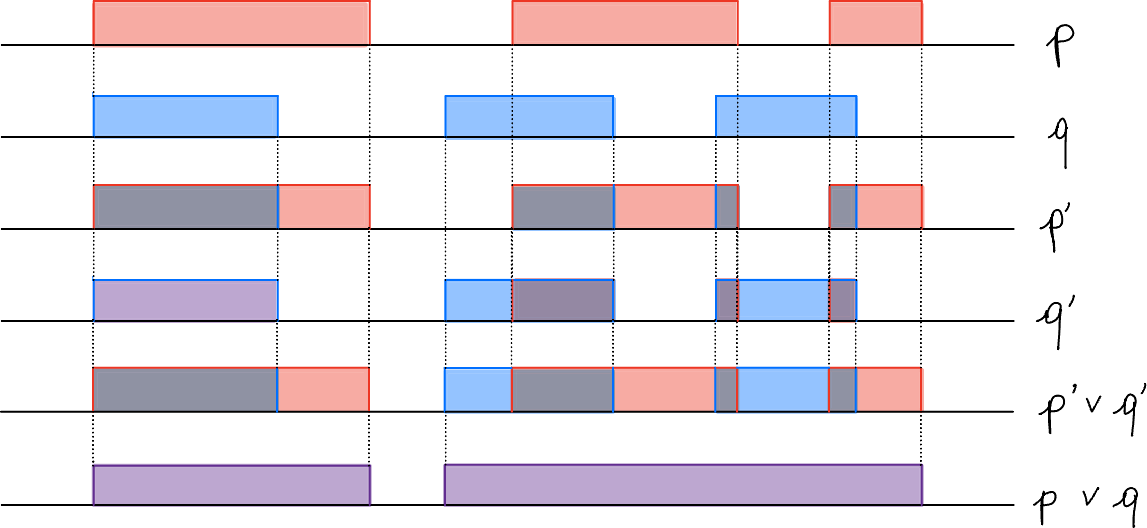
\includegraphics[scale=0.5]{Disjunction.png}

\hspace{1cm}

In the picture the computation process for the interval covering the disjunction. 

\hspace{1cm}

%%%%%%%%%%%%%%%%%%%%%%%%%%%%%%%%%%%%%%%%%%%%% Vedi di inserire l'intervallo per il monitor di until %%%%%%%%%%%%%%%%%%%%%%%%%%%%%%%%%%%%%%

\begin{proposition}
    Let $p$ and $q$ be two unitary signals $\mathcal{I}^+_p=\{I_p\}$ and $\mathcal{I}^+_q=\{I_q\}$. then the signal $\psi=p\,\mathcal{U}_{[a,b]}\,q$ is a unitary signal satisfying $$\mathcal{I}_\psi^+=\{((I_p\cap I_q)\ominus[a,b])\cap I_p\}$$
\end{proposition}

\begin{proof}
    This follows from the semantics of the operator $\mathcal{U}_{[a,b]}$. Consider a point $t\in\{((I_p\cap I_q)\ominus[a,b])\cap I_p\}$. By the semantics of the operator we know that there must be a point $t'\in [a+t,b+t]$ where $q$ and $p$ are satisfied and that $p$ is satisfied also at $t$. Being $p$ unitary, this implies that $p$ holds throughout $[t,t']$. A point $t\not\in I_\psi$ will either not have such a point $t'$ or will not satisfy $p$, and hence not satisfy $\psi$.

\end{proof}

\begin{proposition}
    Let $p=\bigvee_{i=1}^m p_i$ and $q=\bigvee_{j=1}^n q_j$ be two signals each written as a union of unitary signals. Then $$p\,\mathcal{U}_{[a,b]}\,q=\bigvee_{i=1}^m\bigvee_{j=1}^n p_i\,\mathcal{U}_{[a,b]}\,q_j.$$
\end{proposition}

\begin{proof}
    Notice that $p\,\mathcal{U}_{[a,b]}\,(q_1\lor q_2)=p\,\mathcal{U}_{[a,b]}\,q_1\lor p\,\mathcal{U}_{[a,b]}\,q_1$. This holds because $q[t]$ is quantified existentially in the semantic definition. The same holds for $(p_1\lor p_2)\,\mathcal{U}_{[a,b]}\,q$, when the positive intervals are separated. Repeating the reasoning $n$ times for $p$ and $m$ times for $q$ we get the desired result.
    
\end{proof}

These imply correctness of the procedure and that the complexity of it is $O(k\cdot n)$, where $k$ is the number of sub-formulae and $n$ the maximal number of positive intervals in the atomic signals.

\section{REAL-VALUED SIGNALS}

Extend our semantics and logic to real-valued signals. Unlike Boolean and finite variability signals, the real-valued ones do not admit a finite representation. They are represented via sampling that is a sequence of time stamped values of the form $(t,s[t])$. 

For signals of the form $s:\mathbb{T}\to\mathbb{R}^m$ is not possible to ignore issues related to their representation based on output of some numeric simulator.
The logic do not speak about continuous signals but rather of a set of static abstraction from $\mu: \mathbb{R}^m\to\mathbb{B}$. This function create a partition of the continuous state-space according to the satisfaction of some inequality constraints on the real variables. As long as $\mu(s[t])$ is constant we do not care about the exact value of the signal. However, in order to be able to sample the formulae we need to require our sampling to be sufficiently dense, in order to detect the transition. 

The dynamics of most reasonable systems have bounded frequency, and even adding noise, the frequency remains bounded by the size of the integration step by the simulator. We assume we deal with signals that are well-behaving with respect to every $\mu$, which means that:
\begin{itemize}[leftmargin=0.5cm]
    \item $\mu(s)$ has a bounded variability,
    \item every change in $\mu(s)$ is detected, i.e. every point $t$ s.t. $\mu(s[t])\neq\lim_{t'\to t}\mu(s[t'])$ is included in the sampling.
\end{itemize}

\begin{definition}
    Let $U=\{\mu_1,\dots,\mu_n\}$ be a collection of predicates (effective functions) of the form $\mu_i:\mathbb{R}^m\to\mathbb{B}$. Then an $\mathtt{STL}(U)$ formula is an $\mathtt{MITL}_{[a,b]}$ formula over the atomic propositions $\mu_1(x),\dots,\mu_n(x)$.
\end{definition}

Any well-behaved signal with respect to $U$ can be transformed into a Boolean signal $s':\mathbb{T}\to\mathbb{B}^n$ s.t. $s'=\mu_1(s)\|\mu_2(s)\|\dots\|\mu_{n-1}(s)\|\mu_n(s)$ is of bounded variability. By construction, we get that for every \STL formula $\varphi,\, s\vDash\varphi$ iff $s'\vDash\varphi'$ in $\mathtt{MITL}_{[a,b]}$. ($\varphi'$ is obtained by $\varphi$ by replacing every $\mu_i(x)$ with a  propositional variable $p_i$)

The monitoring process is the following:
\begin{enumerate}[leftmargin=0.5cm]
    \item Construction of a Boolean filter for every $\mu_i\in U$, 
    \item Transform $s$ into a Boolean signal, i.e. $p_i=\mu_i(s)$
\end{enumerate}

\b{Ex.} Consider the signal $\sin[t]$ where $t$ is measured in degrees and $\mu(x)=x>0$. The sampling is of length $400$, collecting measure every $50$ time units, plus the collections of the zeros of the function at $180$ and $360$ The input of the Boolean filter is the following:

\begin{gather*}
    (0, 0.0), (50, 0.766), (100, 0.984), (150, 0.5), (180, 0.0), (200, -0.342), \\
    (250, -0.939), (300, -0.866), (350, -0.173), (360, 0), (400, 0.643)\\
\end{gather*}

and the output is the signal $p$ s.t. $\mathcal{I}^+_p=\{[0,180),[360,400)\}$, then we can apply the monitoring described before.

\chapter{\citetitle{donze2013}}

\begin{itemize} [leftmargin=1.25cm]
    \item [\b{Object}:] Presentation of an efficient algorithm for computing the robustness degree in which piecewise-continuous signal satisfies or violates a \STL formula.
\end{itemize}

\TL is a popular formalism used in systems design and formal verification in an either deductive or algorithmic method.  The behaviors studied are typically discrete (sequence of states or events). Problem with the assumption behind \TL use:
\begin{itemize}[leftmargin=0.5cm]
    \item \b{Correctness}: requires that all system behaviors satisfy the specification, thus model checking is based on composing the system model with an automaton for specification and analyzing and all possible paths
    \item \b{Discreteness}: the satisfaction in this logic is purely discrete.
\end{itemize}

New trends in alternative ways of using \TL in designing complex systems, including their operations:
\begin{enumerate}[leftmargin=0.5cm]
    \item \b{Statistical methods a-la Monte Carlo} where universal quantification is replaces with random simulation. 
    \item  \b{Assertion checking or monitoring} where \TL is used as a rigorous specification of the requirements, but it is evaluated on a single behavior at a time. It requires a process that generates observable behaviors. Temporal property checking can be integrated in monitoring and diagnostics of real systems during their operation
\end{enumerate}

\begin{itemize}[leftmargin=2.05cm]
    \item [\b{Monitoring}:] does not require any model, only a process that generates observable behavior. It can be applied to systems as black boxes or to programs without a decent and tractable formal model. The temporal propriety monitoring can be implemented in real systems.
\end{itemize}

In the paper is presented \STL and its monitoring AMT. When dealing with continuous dynamics and numerical quantities, yes/no answers provide only partial information and could be augmented with quantitative information about the satisfaction to provide a better basis for decision-making. 

\b{Ex.} Consider $\varphi: \mathtt{x}<c$ with $c$ constant and $x\in X\subseteq\mathbb{R}$. The formula $\varphi$ we can define a cut on the set in $X_0=\{x\,|\,x\geq c\}$ and $X_1=\{x\,|\,x<c\}$. $X_1$ is called the \b{validity domain} of the formula, since we have that if there is an $x\in X$ s.t. $x\vDash\mathtt{x}<c$, then it means that $x\in X_1$. The robustness degree of a satisfaction should tell us if $x$ satisfies the formula by far or marginally. It captures the $c-x$ and its sign tell us the satisfaction violation of the formula, while its magnitude the robustness. 

In this paper an optimal algorithm that computes robustness is presented. This algorithm guarantees that the over-head added by monitoring to the simulation process is acceptable. It computes in linear time, fo  the following reasons:
\begin{itemize}[leftmargin=0.5cm]
    \item use of the optimal streaming algorithm of Daniel Lemire to compute the extrema of a sequence over an interval,
    \item rewriting of the bounded until operator as a conjunction of an untimed and a simple timed operators.
\end{itemize}

\section{Signal Temporal Logic}
Recall the framework set of \cite{maler2004}  and extension of it to a multivalued logic as proposed in \cite{fainekos2009}. The set of Booleans is defined as follows $\mathbb{B}=\{\bot,\top\}$, with the following proprieties:
\begin{itemize}[leftmargin=0.5cm]
    \item $\bot<\top$,
    \item $-\top=\bot$,
    \item $-\bot=\top$.
\end{itemize}

Consider $\overline{\mathbb{R}}=\mathbb{R}\cup\mathbb{B}$ that is a total-ordered set of real numbers with the smallest element $\bot$ and greatest $\top$. 

A signal is a function $s:\mathcal{D}\to\mathcal{E}$, with $\mathcal{D}\subseteq\mathbb{R}^+_0$ and $\mathcal{E}\subset\overline{\mathbb{R}}$. If $\mathcal{E}=\mathbb{B}$ then $s$ is a Boolean signal, if $\mathcal{E}=\mathbb{R}$ is a real-valued signal. 

A trace $w$ is a set of real-valued signals $\{x_1^w, \dots, x_k^w\}$ defined some interval $\mathcal{D}$, called time domain of $w$. We can transform such trace in a set of predicates of the form $x_i\geq 0$. \STL is an extension of Metric Temporal Logic using real-valued signals. 

\begin{align*}
    \textbf{Syntax:}    &\quad\varphi:=\top\,|\,x_i\geq0\,|\,\lnot\varphi\,|\,\varphi_1\land\varphi_2\,|\,\varphi_1\lor\varphi_2\,|\,\varphi_1\mathcal{U}_{[a,b]}\varphi_2
\end{align*}

Let $w$ be a trace of time domain $\mathcal{D}$. The formula $\varphi$ is said defined over a time interval $\dom{\varphi}$, define recursively on the complexity of $\varphi$ as follows:
\begin{align*}
    \dom{\top}=                          &\;\dom{x_i\geq0}=\mathcal{D},\\
    \dom{\lnot\varphi}=                  &\;\dom{\varphi},\\
    \dom{\varphi\land\psi}=              &\;\dom{\varphi}\cap\dom{\psi},\\
    \dom{\varphi\lor\psi}=               &\;\dom{\varphi}\cup\dom{\psi},\\
    \dom{\varphi\,\mathcal{U}_{[a,b]}\,\psi}=  &\;\{t \in \mathbb{R} \,|\, t, t + \inf[a, b]\in \dom{\varphi}\text{ and } \\ & \;\;\,t + \inf[a, b] \in \dom{\psi}\}.
\end{align*}

\subsection{Boolean semantics}
Now, we can define the Boolean semantics. Given a trace $w$, the validity of a \STL formula $\varphi$ at a time $t\in\dom{\varphi}$, is defined inductively as follows:
\begin{align*}
    w,t\vDash \text{true} \quad\quad                                                  &\\
    w,t\vDash x_i\geq 0 \quad                               \Leftrightarrow    &\quad x_i^w(t)\geq 0\\
    w,t\vDash \lnot \varphi \quad                           \Leftrightarrow    &\quad w,t\nvDash \varphi \\
    w,t\vDash \varphi \land \psi \quad                      \Leftrightarrow    &\quad w,t\vDash \varphi \text{ and } w,t\vDash \psi\\
    w,t\vDash \varphi \lor \psi  \quad                      \Leftrightarrow    &\quad w,t\vDash \varphi \text{ or } w,t\vDash \psi\\
    w,t\vDash \varphi \, \mathcal{U}_{[a,b]} \, \psi \quad  \Leftrightarrow    &\quad \exists t'\in [a+t,b+t], w,t'\vDash\psi \,\text{ and }\, \forall t''\in[t,t']w,t''\vDash\varphi_1[t'']
\end{align*}

All the abbreviations are valid as well as the definitions for $\nec_{[a,b]}\varphi$ and $\pos_{[a,b]}\varphi$. We have also the untimed operator that are timed operators over the interval $[0,\infty)$. Then we give also the following definition: $$\text{false} = \lnot\text{true}.$$

For a given formula $\varphi$ and a trace $w$, we define the \b{satisfaction signal} $\chi(\varphi,w,\bullet)$ as follows:

\begin{align*}
    \text{for all } t\in\dom{\varphi},  &\quad\chi(\varphi,w,t)=\begin{cases}
                                                                    \top    &\text{if } w,t\vDash\varphi,\\
                                                                    \bot    &\text{otherwise}.
                                                                 \end{cases}
\end{align*}

Monitoring the satisfaction of a formula $\varphi$ can be done by computing for each subformula the entire satisfaction signal $\chi(\varphi,w,\bullet)$, following the procedure described in \cite{maler2004}.

\subsection{Quantitative semantics}

Given a formula $\varphi$, a trace $w$ and a time $t\in\dom{\varphi}$, we define the quantitative semantics $\rho(\varphi, w, t)$ inductively as follows:

\begin{align*}
   \rho(\text{true},w,t) \quad                          =   &\quad \top\\
   \rho(x_i\geq 0,w,t) \quad                            =   &\quad x_i^w(t)\\
   \rho(\lnot \varphi,w,t) \quad                        =   &\quad -\rho(\varphi,w,t) \\
   \rho(\varphi \land \psi,w,t) \quad                   =   &\quad \min\{\rho(\varphi,w,t),\rho(\psi,w,t)\}\\
   \rho(\varphi \lor \psi,w,t) \quad                    =   &\quad \max\{\rho(\varphi,w,t),\rho(\psi,w,t)\}\\
   \rho(\varphi \, \mathcal{U}_{[a,b]} \, \psi) \quad   =   &\quad \sup_{t'\in[a+t,b+t]}\min\biggl\{\rho(\psi,w,t'), \inf_{t''\in[t,t']}\rho(\varphi,w,t'')\biggr\}
\end{align*}

If we define $\chi(x_i>0,w,t)$, applying the definition above and we apply it to the inductive definition of $\rho$ we get back to Boolean signals and obtain again $\chi$.

In this type of semantics however, atomic predicates do not evaluate $\top$ or $\bot$, but give a real value representing the distance to satisfaction or to violation and propagate it to the formula using operations on $\overline{\mathbb{R}}$.

For the lattice proprieties of $(\overline{\mathbb{R}},<)$ we are granted the associativity, commutativity, neutral element and distributivity. Minus function is involutive, which gives the propositional and the modal version of de Morgan laws:
\begin{align*}
    \lnot(\varphi\lor\psi) \quad\equiv  &\quad \lnot\varphi\land\lnot\psi\\
    \lnot\pos_{[a,b]}\varphi \quad\equiv  &\quad \nec_{[a,b]}\lnot\varphi
\end{align*}

Therefore, we have for the derived operators the same natural interpretations:

\begin{align*}
    \rho(\pos_{[a,b]}\varphi,w,t) \quad =   &\quad\sup_{t'\in[a+t,b+t]}\rho(\varphi,w,t')\\
    \rho(\nec_{[a,b]}\varphi,w,t) \quad =   &\quad\inf_{t'\in[a+t,b+t]}\rho(\varphi,w,t')
\end{align*}

\subsection{Propriety of Robustness Estimate}

The quantitative semantics of \STL have two proprieties, that would alone justify their introduction. 

If $\rho(\varphi,w,t)\neq0$, its sign indicates the satisfaction status.

\begin{proposition}[Soundness]
    Let $\varphi$ be a \STL formula, $w$ a trace and a $t$ time. Then 
    \begin{align*}
        \rho(\varphi,w,t)>0\quad   \Rightarrow  &\quad w,t\vDash\varphi
    \end{align*}
\end{proposition}

If $w$ satisfies $\varphi$ at time $t$, any other trace $w'$  whose pointwise distance from $w$ is smaller than $\rho(\varphi),w,t$ also satisfies $\varphi$ at time $t$.

\begin{proposition}(Correctness)
    Let $\varphi$ be an \STL formula, $w$ and $w'$ traces over the same time domain, and $t\in\dom{\varphi}$. Then
    \begin{align*}
        w,t\vDash\varphi \,\text{ and }\, \|w-w'\|_\infty<\rho(\varphi,w,t)\quad    \Rightarrow &\quad w',t\vDash\varphi     
    \end{align*}           
\end{proposition}

Given the soundness and the correctness, for a given trace $w$, and a \STL formula $\varphi$, we have that a \b{robustness signal} of $\varphi$ w.r.t. $w$, $\rho(\varphi,w,\bullet)$, is defined over the domain $\dom{\varphi}$.

\subsection{Rewriting the operator Until}
We can claim about the until operator the following proprieties, extended from the Boolean to the quantitative semantics:
\begin{align}
    \varphi \,\mathcal{U}_{[a,b]}\,\psi\quad    \equiv  &\quad\pos_{[a,b]}\psi\:\land\:\varphi\,\mathcal{U}_{[a,+\infty)}\,\psi \label{1}\\
    \varphi\,\mathcal{U}_{[a,+\infty)}\,\psi\quad   \equiv  &\quad\nec_{[0,a]}(\varphi\,\mathcal{U}\,\psi)
\end{align}

\begin{proof} \textcolor{white}{---}

    \b{(\ref{1})}

    Let be $y,y'$ the robustness signals $\varphi, \psi$ relative to $w$. Now consider 
        \begin{align*}
            u=\sup_{\tau\in[a+t,b+t]}\min\biggl\{y'(\tau), \inf_{[t,\tau]}y\biggr\} &\quad \text{and}\\ v=\min\biggl\{\sup_{[a+t,b+t]}y',\sup_{\tau\geq t+a}\min\biggl\{y'(\tau),\inf_{[t.\tau]}y\biggr\}\biggr\}
        \end{align*}
    and let then be the robustness values of the first equivalence for some given $t$.

    Suppose $u\neq v$. Then we define the signals 
    \begin{align*}
        x\::\:t\mapsto y(t)-\frac{u+v}{2} \quad \text{and}  &\quad x'\::\:t\mapsto y'(t)-\frac{u+v}{2}
    \end{align*}

    Let be the formualae
    \begin{align*}
        \gamma=(x\geq0)\,\mathcal{U}_{[a,b]}(x'\geq 0) \quad \text{and}  &\quad \vartheta = \pos_{[a,b]} (x\geq0)\land(x\geq0)\,\mathcal{U}_{[a,+\infty)}(x'\geq 0)
    \end{align*}
\end{proof}
It is possible to push the constant outside the scope of the operators of $\min, \sup,\inf$. Doing this we get their quantitative semantics:

\begin{align*}
                                    &\quad\rho(\gamma, w, t) = v - \frac{u + v}{2} < 0      &\quad \text{and} \quad     & \rho(\vartheta, w, t) = v - \frac{u + v}{2} > 0 \\
\xRightarrow{\text{By Soundness}}   &\quad w, t \nvDash \gamma                              &\quad \text{and} \quad     & w, t \vDash \vartheta
\end{align*}

\section{Computing the Robustness Estimate}

In monitoring signals are available as finite timed over an alphabet $\mathbb{R}^n$, and they can be interpreted as linear interpolation. Presentation of the basic framework for computing robustness, under this hypothesis. 

\begin{algorithm}[H]
    \caption{Robustness($\varphi$, $w$)}
    \Switch{$\varphi$}{
      \Case{$\mathtt{true}$}{
        \Return{$\overline\top \quad \%$ a constant $\overline\top$ signal}\;
      }
      \Case{$x_i \geq 0$}{
        \Return{$x_i^w$}\;
      }
      \Case{$\odot \, \varphi_1$}{
        $y \gets \text{Robustness}(\varphi_1, w)$\;
        \Return{$\mathrm{Compute}(\odot, y)$}\;
      }
      \Case{$\varphi_1\,\odot\, \varphi_2$}{
        $y \gets \text{Robustness}(\varphi_1, w)$\;
        $y' \gets \text{Robustness}(\varphi_2, w)$\;
        \Return{$\mathrm{Compute}(\odot, y, y')$}\;
      }
    }
\end{algorithm}

\begin{definition}
    A signal $y$ is said to be \b{finitely piecewise-linear, continuous} ($\mathtt{f.p.l.c.}$) if there exists a finite sequence $(t_i)_{i\leq n_y}$ s.t.:
    \begin{itemize}[leftmargin=0.5cm]
        \item y is defined over the domain $[t_0,t_{n_y})$,
        \item for all $i<n_y,y$ is continuous at $t_i$ and offline on $[t_i,t_{i+1})$
    \end{itemize}
    $(t_i)_{i\leq n_y}$ is called the \b{time sequence} of $y$.
\end{definition}

Let be $\partial y(t)=\frac{\partial}{\partial t}y(t)$. Any signal in the observed trace will be assumed to be $\mathtt{f.p.l.c.}$, and will be represented by the sequence $(t_i,y(t_i),\partial y(t_i))_{i<n_y}$, along with the cut-off time $t_{n_y}$. 

The representation is redundant, by continuity, but facilitates the splitting into segments. The quantitative semantics preserves the $\mathtt{f.p.l.c.}$ proprieties of the signal. Continuity is preserved over the operators $\sup$ and $\inf$, and no new derivative value is created in the process.

\subsection{Boolean operators}

Computing the robustness of $\lnot \varphi$ from $\varphi$ is trivial. Note that if the sequence $(t_i,y(t_i),\partial y(t_i))_{i<n_y}$ represents $\rho(\varphi,w,\bullet)$ then the sequence $(t_i,-y(t_i),-\partial y(t_i))_{i<n_y}$ represents $\rho(\lnot\varphi,w,\bullet)$.

For conjunction let take $y$ and $y'$ as the robustness of $\varphi$ and $\psi$ respectively, producing $z$ the robustness signal of $\varphi\land\psi$. Then consider the sequence $(r_i)_{i\leq n_z}$ containing the sampling points of $y$ and $y'$ when they are both defined, and the points where $y$ and $y'$ intersect.

\printbibliography
\end{document}